\documentclass[a4paper]{article}

\usepackage[american]{babel}
\usepackage{amssymb}
\usepackage{array}
\usepackage{tabularx}
\usepackage{graphicx}

\usepackage{amsmath}
\usepackage{url}
\usepackage{minted}
\usepackage{float}

\newcommand{\rust}[1]{\mintinline{rust}{#1}}

\begin{document}

\title{{Folley: real-time mosquito noise origin locator} \\\large {Report of the 5LIU0 DBL project}}
\author{{Henk Oordt} \hfill
\\
{1717510} \hfill}
\maketitle
\begin{figure}[H]
    \begin{center}
        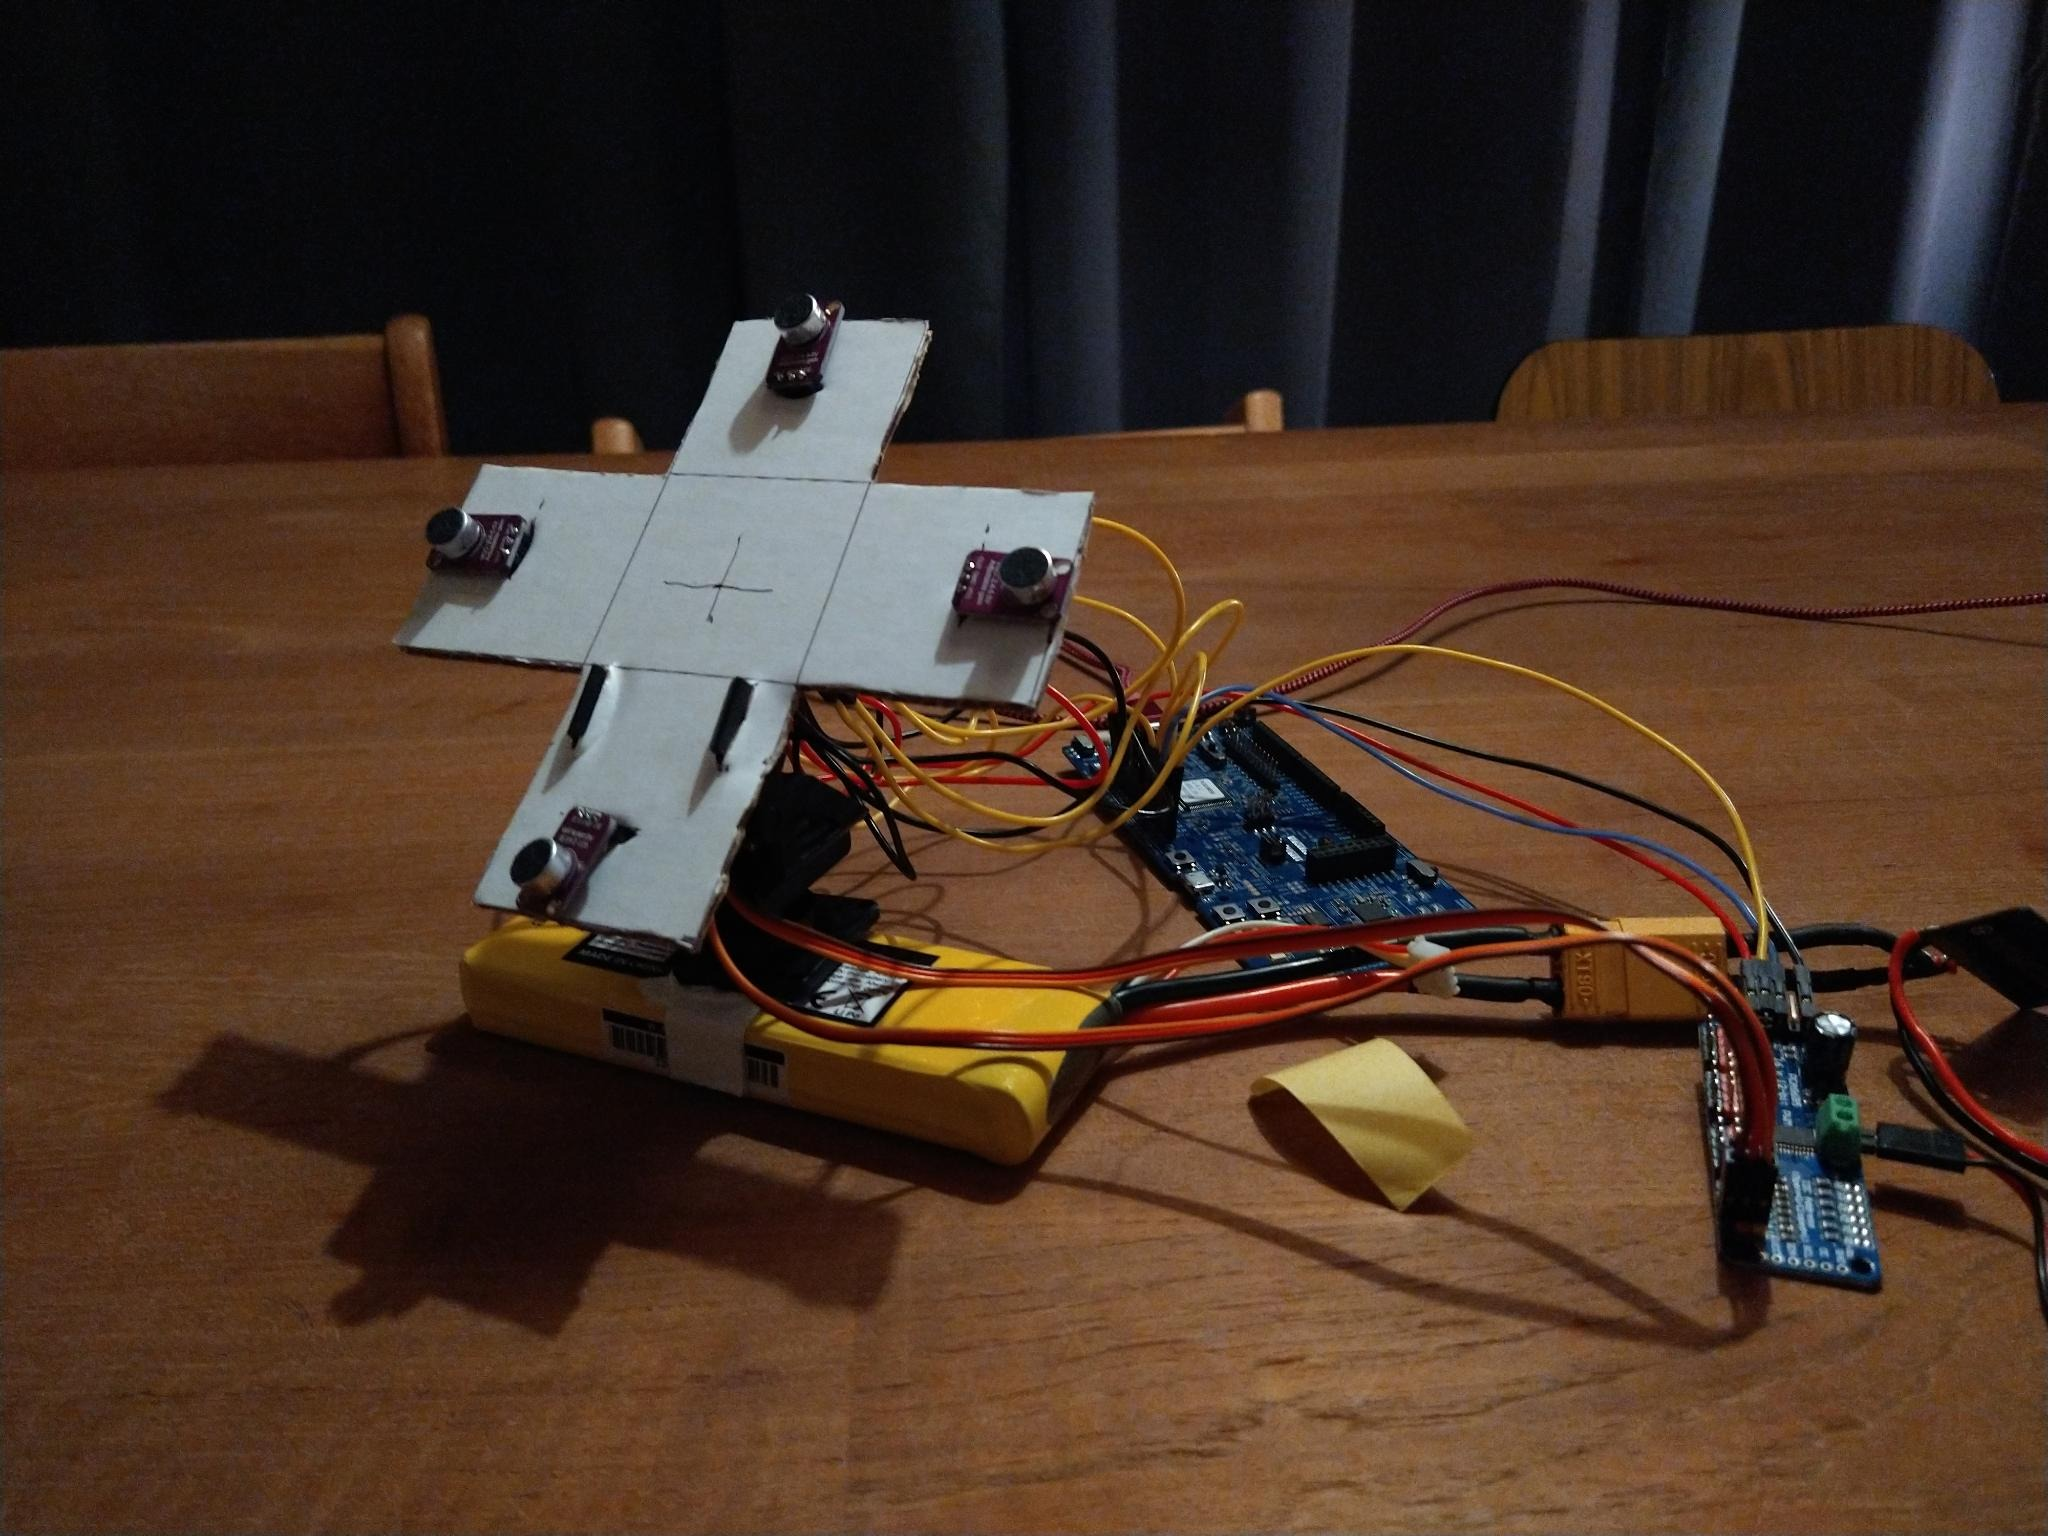
\includegraphics[width=\linewidth]{assets/device.jpeg}
    \end{center}
\end{figure}


\newpage

\section{Introduction}
% A general description of your project and its challenges.
Project `Folley' is aimed at the design and construction of a real-time sound origin locator. Folley uses audio signal analysis to detect and locate in 3D space the origin of the buzzing sound of mosquitoes.

In order to locate the sounds origin, Folley samples audio signal from an array of four analog microphones. The sampled signals are then analyzed in order to calculate a time-delay-angle-of-arrival (TDOA) \cite{6327613} which, along with the known microphone setup dimensions, can be used to calculate the azimuth and altitude angles of the origin with respect to the microphone array of the device.

In order to develop the TDOA analysis software, a set of Matlab \cite{matlab} scripts were written, which given the raw audio signal measurements, can calculate the azimuth and altitude angles of the sounds origin with respect to the microphone array. Essentially, in these scripts all of the signal analysis calculations that are needed to reach the project goals are implemented. These Matlab scripts will serve as a basis and a means of verification for the Rust implementation of the algorithm in firmware. Upon completion of the Matlab scripts and tweaking of parameters, the calculations have been re-implemented in Rust \cite{rust}, in order for the analysis to be done by the microcontroller on the nRF52840 DK \cite{nrf52840-dk} board in real time. A simple command line application written in Rust that can communicate with the device and that converts raw microphone measurements to Matlab input files was developed as well.

This project focuses solely on the implementation of the TDOA analysis, as well as its evaluation. In this project, a testing environment was set up. This environment consists of a simple firmware application that is able to sample microphone data, and communicate these samples with the command line application that records them. The environment having been set up, a Matlab script has been implemented that is able to do the TDOA analysis based on four sine waves with separate phase differences, but with the same frequencies. Once this Matlab script had finished, the TDOA analysis was re-implemented in firmware, so that it can be done with microphone samples in real time. With the this project done, Folley should be able to locate origins of prefedined sine wave sounds, coming from a waveform generator, as well as recordings of real mosquito buzzing sound.

\textit{The software developed in this project, as well as the data used to verify calculations, are available online within the project repository \cite{repo} an in the accompanying archive. This report references paths within the archive and repository.}

\section{Problem specification}
% A detailed and technical description of the problem you’re addressing.
Mosquitos emit a continuous buzzing sound in which certain frequencies and harmonics are present when flying around. This sound can be used to estimate the location of the insect. A device can use a set of microphones to analyze the sound signals as it is recorded by multiple microphones and obtain information about the location of the insect.

\begin{figure}[H]
    \begin{center}
        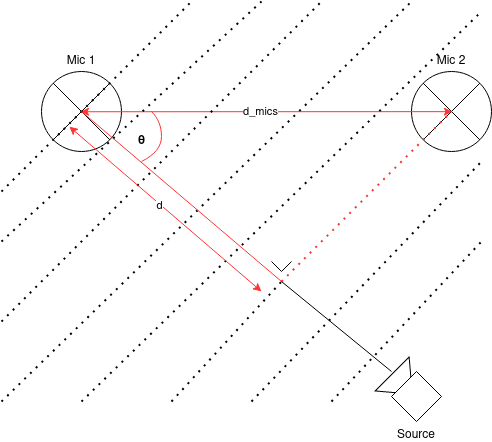
\includegraphics[width=25em]{assets/problem_overview.png}
        \caption{Problem overview}
        \label{fig:problem_overview}
    \end{center}
\end{figure}

As the insect moves, the sound will come from different angles from the device perspective. For both the x and y axis, the time of arrival of the buzzing sound can be used to calculate the angle from which it originated. In figure \ref{fig:problem_overview}, a schematic overview of the problem is given for a single axis. A sound source produces a sound. The origin is assumed to be infinitely far away, so the sound is moving in straight waves when it arrives at the microphone array. In this example, the sound hits microphone 2 before it hits microphone 1. Let $d$ be the distance travelled by the sound between the moment it hits microphone 2 and the moment it hits microphone 1 and $d_{mics}$ be the distance between the microphones. Then, a right triagle can be formed with a hypotenuse of length $d_{mics}$, one side of length $d$ and an angle $\theta$ between them. In order for $\theta$ to be calculated, the following equation is used:\[\theta = \arctan(\frac{d}{d_{mics}})\] $\theta$ equals the angle between the device and the sound origin. $\theta$ ranges from $0^{\circ}$ to $90^{\circ}$ to $180^{\circ}$ as the source is moved from the right, to the middle, towards the left of the array.

Given the delay $t_{delay}$ in time between the moment the sound hits microphone 1 ($t_1$) and the it hits moment microphone 2 ($t_2$), with $t_{delay} = t_1 - t_2$ $d$ can be derived as follows:\[d = t_{delay} \cdot V_{sound}\]where $V_{sound}$ is the speed of sound, $343\ m/s$

The challenge for this project is to find $t_{delay}$ given just the raw microphone samples from ADC of the microcontroller. This process is called Time Delay angle Of Arrival (TDOA) analysis.


To estimate $t_{delay}$, we can use cross-correlation of two signals. Using cross-correlation, the precense of one signal can be detected within another signal. It is a measure of similarity between two signals as one signal is delayed with respect to the other. For discrete signals, cross correlation between real-value signals $x$ and $y$ is defined as follows: \[(x \star y)[n] \triangleq \sum_{m = -\infty}^ {\infty} x[m]\cdot y[m + n]\] This yields a new signal, of which the $n$ corresponding the highest value is the delay between the signals for which they were most similar. Therefore, the delay between the signals $x$ and $y$ in terms of number of samples, $n_{delay}$ can be found with \[n_{delay} = \underset{n}{\mathrm{argmax}}\ (x \star y)[n]\] Given a fixed sample period $T_s$ used for both signals, $t_{delay}$ can be calculated with \[t_{delay} = n_{delay} \cdot T_s\]

$t_{delay}$ has a maximum at $\theta = 180^{\circ}$ and a (negative) minimum at $\theta = 0^{\circ}$. Therefore, the calculations can be optimized by only calculating the cross correlation for a limited range of $n$. The upper limit of $n$, $n_{max}$, can be found by \[n_{max} = \frac{d_{mics}}{T_s \cdot V_{sound}}\] The minimum is found by $n_{min} = -n_{max}$. Given these limits, the length of the cross correlation signal can be reduced drastically:\[(x \star y)[n] \triangleq \sum_{m = n_{min}}^ {n_{max}} x[m]\cdot y[m + n]\]

If the wave length $\lambda$ is no greater than $d_{mics}$, using the limited cross correlation also makes the cross correlation suitable for periodic sigals: the signals will only optimally lined up for one value of $n$. Therefore, a suitable value for $d_{mics}$ needs to be found in order for the device to be able to work with typical mosquito buzzing sound, keeping in mind its periodicity. This is done by analyzing the Fourier transform a mosquito buzzing sound fragment\cite{mosquito_fragment}, as from it can be obtained the sound's fundamental frequency $f_0$. With $f_0$ determined, $\lambda$, and therefore $d_{mics}$, can be found with \[\lambda = \frac{V_{sound}}{f_0}\]

This completes the set of calculations needed to calculate $\theta$ given two signals. In this project, the before calculations were implemented in order to find a suitable value for $d_{mics}$, and for the TDOA analysis to efficient enough for them to be done on-device in real time.

\section{Evaluation criteria}
% How will you be able to determine if your project is successful? Try to find objective and quantitative metrics.
In order to indicate whether the device can locate a mosquito successfully, the following goal is defined. Firmware should be able to calculate the azimuth angle of a sound origin within a 10 degree error margin 80\% of the time, when presented with a predefined sine wave as sound signal, as well as a real mosquito sound fragment.
% TODO speed goal

\section{Setup}
% What are the signals (real, simulated or physical) that you will use for your project? What is the hardware and/or software setup that you have used?

To find a suitable value for $d_{mics}$, a Fourier transform of a mosquito sound fragment \cite{mosquito_fragment} was done. In figure \ref{fig:mosquito_fourier}, a plot of this transform was done. From the figure, it can be concluded that the sound signal in the analyzed fragment has a base frequency of about $367$ Hz. Also, some strong harmonics can be found at $f_1 = 730\ Hz$ and $f_2 = 1102\ Hz$. The length of a full period is therefore determined as $\lambda = \frac{V_{sound}}{f_0} = \frac{343}{367} = 0.9\ m$. For our device to be able to work with this periodic mosquito sound, a value of $d_{mics} = 125\ mm$, which is significantly smaller than $\lambda$, is sufficient.

\begin{figure}[H]
    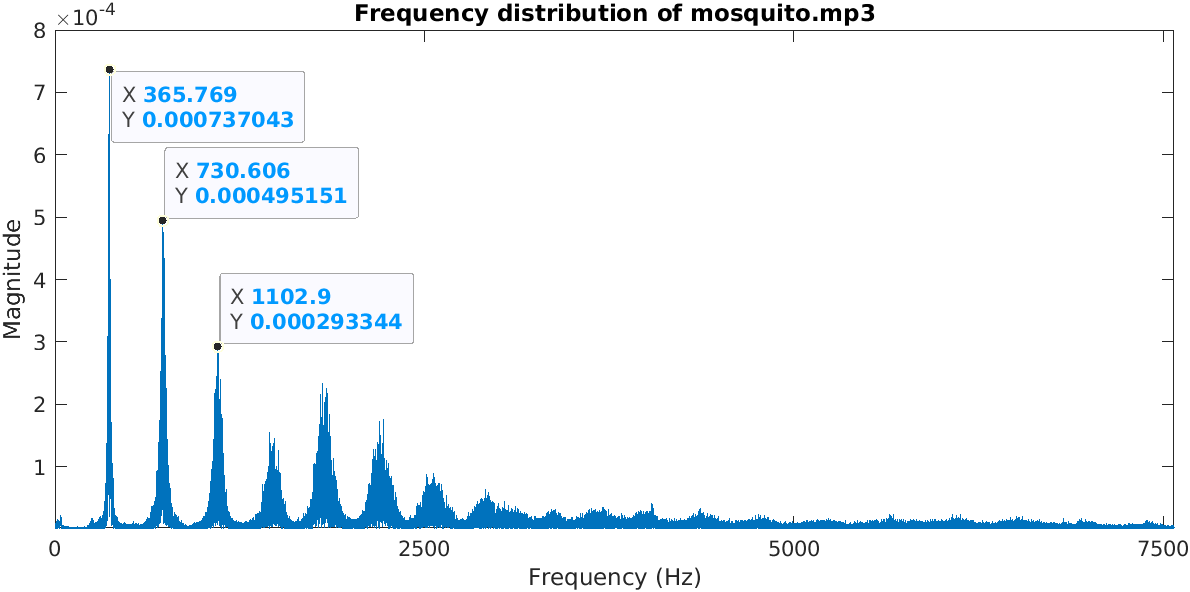
\includegraphics[width=34em]{assets/mosquito_fourier.png}
    \caption{Fourier transform of mosquito.mp3}
    \label{fig:mosquito_fourier}
\end{figure}

The device is controlled by a Nordic Semiconductor nRF52840 microcontroller \cite{nrf52840}, mounted on a nRF52840DK board, for which firmware is customly written in Rust \cite{rust}.  The nRF52840 microcontroller is able to sample up to 8 analog inputs. Having four analog input channels enabled with an aquisition time of $5\ \mu s$, it is able to sample with a minimal sample period of $ T_s = 22\ \mu s$. As the on-chip ADCs can be controlled by timer peripherals directly, the sample period can be configured with great flexibility. The nRF52840dk board can also relatively easily be set up for serial communication over USB \cite{usb}, enabling running real-time analysis and graph plotting on a host computer for development ease. What's more, using defmt \cite{defmt}, data can be easily logged to the host device when attached to a debugger. This proves useful when obtaining raw samples or TDOA analysis results from the device.

\begin{figure}[H]
    \begin{center}
        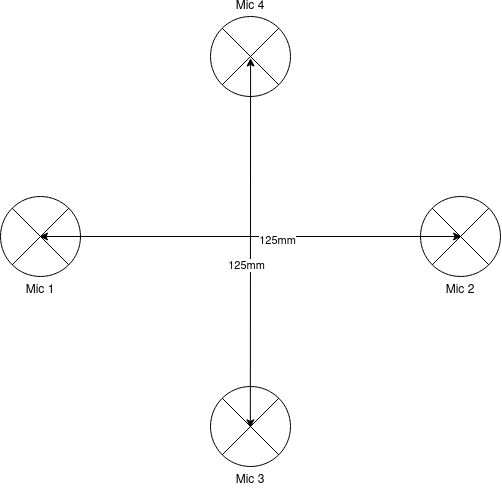
\includegraphics[width=25em]{assets/mic_array_dimensions.png}
        \caption{Microphone array dimensions}
        \label{fig:mic_array_dimensions}
    \end{center}
\end{figure}

The device uses an array of four electret microphones, mounted in a `+'-shape. As can be seen in figure \ref{fig:mic_array_dimensions}, every two opposite microphones are $125\ mm$ apart. Using this setup, it becomes possible to esimate the angle from which the buzzing sound comes from in both the horizontal and vertical axis. In this project, however, only the analysis of a single axis is benchmarked, as the accuracy of the second axis is expected to be very similar because of $d_{mics}$ being equal for both axes.

The actual signals the device has to deal with are the analog microphone output voltages, being amplified by an op-amp integrated in each microphone module. As the device uses the ADC integrated in the nRF52840, the software handles obtained from the ADC peripheral. The ADC peripheral can be assigned a block of memory with a customizable size. It can be configured to trigger an interrupt whenever the block is full, in order for the samples to be processed further. In this project, is is configured to produce 12-bit 2's complement integer values, with a sample period of $T_s = 37 \mu s$. A suitable sample period was found by trial and error.

To manage the tasks the microcontroller has to fulfill in order to configure its peripherals, fetch and analyze samples and communicate, the device firmware is written with the RTIC framework \cite{rtic}. This framework uses dynamic interrupt prioritization to schedule and pre-empt tasks. This framework is based om the Rust programming language, in which all of the firmware is written. Among many others, a trait of Rust is that it is very easy to write and compile platform-independent code. This enables us to test and validate firmware modules on a PC. The device firmware is available in the \texttt{./prototype/firmware} directory.

Another part of the project is the implementation of a command-line interface (CLI) application that can communicate with the device firmware over UART, the source of which is present in the \texttt{./prototype/cli} directory. Code in modules and libraries written in Rust also be shared between multiple applications, enabling for easily defining a shared communication format, which has been done in this project. Its source code can be found in the \newline\texttt{./prototype/format} directory. Using this communication format, the CLI is able to send commands to the device as well as receive raw samples from it. These raw samples can be logged to a file which matlab is able to read using its `readmatrix' command. Using the logged raw samples, Matlab scripts have been developed with which all calculations described in the problem specification are automated and can be found in the \texttt{./matlab} folder. These scripts are able to do the full TDOA analysis, given a file of raw measurements.

The Matlab script output is used as a basis for re-implementing the calculations in Rust, for them to be run on-device and in the CLI. These calculations are implemented in this \rust{folley-calc} package, which is present in the \texttt{./prototype/calc} folder. This package is used by both the firmware and the CLI application to do analysis of raw samples, and contains unit tests that verify the calculations using output of the Matlab scripts for a recorded set of samples. As the \rust{folley-calc} package is at the heart of the firmware application, some parts of this package is discussed in more detail in the following section.

\section{Approach}
% A detailed, technical description how you solved the problem.

The \texttt{folley-calc} package contains multiple functions that together implement all calculations needed to estimate the location of a sound-producing object given a set of samples. In listing \ref{list:xcorr_real_impl}, a snippet of the implementation of the cross correlation is given. In this snippet, \rust{SIGNAL_LEN} is the length of the signals \rust{x} and \rust{y}. In the firmware application, the value of \rust{XCORR_LEN} is calculated by $XCORR\_LEN = 2 * n_{max} + 1$, and is thus dependent on the distance between the two microphones the signals were obtained from and the sample period $T_s$. The result of the cross correlation is stored in the \rust{out} array, and the index for which the output signal has the greatest value, \rust{argmax} is returned at the bottom. As indexing arrays with negative indices is not suppported in Rust, the actual lag $n_{delay}$ is obtained by \rust{argmax - (XCORR_LEN as isize / 2);}. As the value of \rust{y[y_index]} might not always be defined, it defaults to $0$.

\begin{listing}[H]
    \begin{minted}[autogobble]{rust}
        //snip ...
        let mut argmax = 0;
        let mut max = 0;
        for n in 0..XCORR_LEN {
            for m in 0..SIGNAL_LEN {
                let x_val = x[m] as i64;
                let y_index = (n + m) as isize - (XCORR_LEN as isize) / 2;
                let y_val = if y_index >= 0 {
                    *y.get(y_index as usize).unwrap_or(&0)
                } else {
                    0
                } as i64;
                out[n] += x_val * y_val;
            }
            if out[n] > max {
                max = out[n];
                argmax = n;
            }
        }
        argmax
        //snip ...
    \end{minted}
    \caption{Implementation of the cross correlation of signals x and y in \rust{folley_calc::xcorr_real}}
    \label{list:xcorr_real_impl}
\end{listing}

With $n_{lag}$ having been obtained, the next part is calculating the angle, given $d_{mics}$ and $T_s$. This calculation involves geometrical calulations, which are typically slow on embedded devices. To mitigate this, a lookup table can be generated using the \rust{foley_calc::gen_lag_table}. The generated table contains tuples in which $n_{delay}$ is mapped to an angle in degrees. In listing \ref{list:lag_table} a snippet from an example lag table is given. The idea is that the lag table is generated only once at application start, and is used to look up angles corresponding to values for $n_{delay}$.

\begin{listing}[H]
    \begin{minted}[autogobble]{rust}
        //snip ...
        (-4, 99),
        (-3, 97),
        (-2, 95),
        (-1, 93),
        (0, 90),
        (1, 88),
        (2, 86),
        (3, 84),
        (4, 82),
        //snip ...
    \end{minted}
    \caption{Snippet of a lag table as generated by \rust{folley_calc::gen_lag_table} with $T_s = 14\ \mu s$ and $d_{mics} = 125\ mm$}
    \label{list:lag_table}
\end{listing}

Listing \ref{list:on_samples} is an excerpt of the \newline\rust{folley_firmware::on_samples} firmware task, which receives the samples from ADC, calls the TDOA analysis function \rust{folley_calc::calc_angle}, to obtain angles for two sets of microphones. The values for the contants passed to the \rust{calc_angle} function are given in listing \ref{list:consts}. From these values can be derived that the amount of samples in each of the compared signals is 1024. In other words, every TDOA analysis cycle is done with two signals containing 1024 raw samples, sampled with a sample period of $T_s = 37\ \mu s$. The firmware task prints the output using defmt to the console of the debugging host. An excerpt of example output is given in listing \ref{list:defmt_output}. During the evaluation experiment, only the values for the x-axis is reported, as the values for the y-axis are obtained in exactly the same manner. To analyze the measurements, the defmt output is stripped of anything not being the x-axis output. This yields a list of just the calculated angles for the x-axis.

\begin{listing}[H]
    \begin{minted}[autogobble]{rust}
        //snip ...
        let mut buf = [0i64; MAX_LAG];
        let x_angle = folley_calc::calc_angle::<
            T_S_US, 
            D_MICS_MM, 
            MAX_LAG, 
            SAMPLE_BUF_SIZE
        >(
            &channels.ch1,
            &channels.ch2,
            &mut buf,
            ctx.resources.lag_table,
        ) as i32;
        let y_angle = folley_calc::calc_angle::<
            T_S_US, 
            D_MICS_MM, 
            MAX_LAG, 
            SAMPLE_BUF_SIZE
        >(
            &channels.ch3,
            &channels.ch4,
            &mut buf,
            ctx.resources.lag_table,
        ) as i32;
        defmt::info!("x: {}\t\ty: {}", x_angle, y_angle);
        //snip ...
\end{minted}
    \caption{Snippet of \rust{folley_firmware::on_samples}}
    \label{list:on_samples}
\end{listing}

\begin{listing}[H]
    \begin{minted}[autogobble]{rust}
        pub mod consts {
            use folley_calc::max_lags_size;

            /// Sample period in microseconds
            pub const T_S_US: u32 = 37;
            /// Distance between two mics in millimeters
            pub const D_MICS_MM: u32 = 125;

            /// Size of a set of samples
            pub const SAMPLE_BUF_SIZE: usize = 1024;
            /// Amount of lags evaluated in the cross correlation
            pub const XCORR_LEN: usize = max_lags_size(T_S_US, D_MICS_MM);
        }
    \end{minted}
    \caption{Snippet of \rust{folley_firmware::consts}}
    \label{list:consts}
\end{listing}

\begin{listing}[H]
    \begin{minted}[autogobble]{bash}
        25 INFO  x: 102    y: 90
        26 INFO  x: 90     y: 90
        27 INFO  x: 90     y: 90
        28 INFO  x: 90     y: 90
        29 INFO  x: 90     y: 90
        30 INFO  x: 114    y: 90
        31 INFO  x: 90     y: 90
        32 INFO  x: 90     y: 90
        33 INFO  x: 90     y: 90
        34 INFO  x: 108    y: 90
        35 INFO  x: 90     y: 90
        36 INFO  x: 90     y: 90
        37 INFO  x: 90     y: 90
        38 INFO  x: 90     y: 90
        39 INFO  x: 102    y: 85
    \end{minted}
    \caption{Example defmt output of the \rust{folley_firmware::on_samples} task}
    \label{list:defmt_output}
\end{listing}

The actual evaluation test is done by placing the microphone array next to a speaker at a distance of about $50\ cm$, as can be seen in figure \ref{fig:test_setup}. The speaker is placed at angles of $\theta = 0^{\circ}$, $\theta = 45^{\circ}$, $\theta = 90^{\circ}$, $\theta = 135^{\circ}$, and $\theta = 180^{\circ}$ from the horizontal microphone array. At each angle, the mosquito buzzing sound sample used in the Fourier analysis in section 4 is played from the speaker, as well as a sine wave noise of 1100Hz. The resulting log files are then analyzed in the Matlab function shown in listing \ref{list:analyze_measurements}. To it is passed the file name to analyze, as well as the angle $\theta$ at which the speaker was placed. The function calculates and prints the number of calculation outputs in the file, the average estimated angle, the standard deviation of the output, the amount and percentage of values that were within a $10^{\circ}$ margin from the expected angle, and whether the test was passed for the current list of outputs. As a baseline, a set of ouputs is analyzed with the speaker off as well. The values obtained from this analysis are discussed in the next chapter.

\begin{figure}[H]
    \begin{center}
        % TODO new pic
        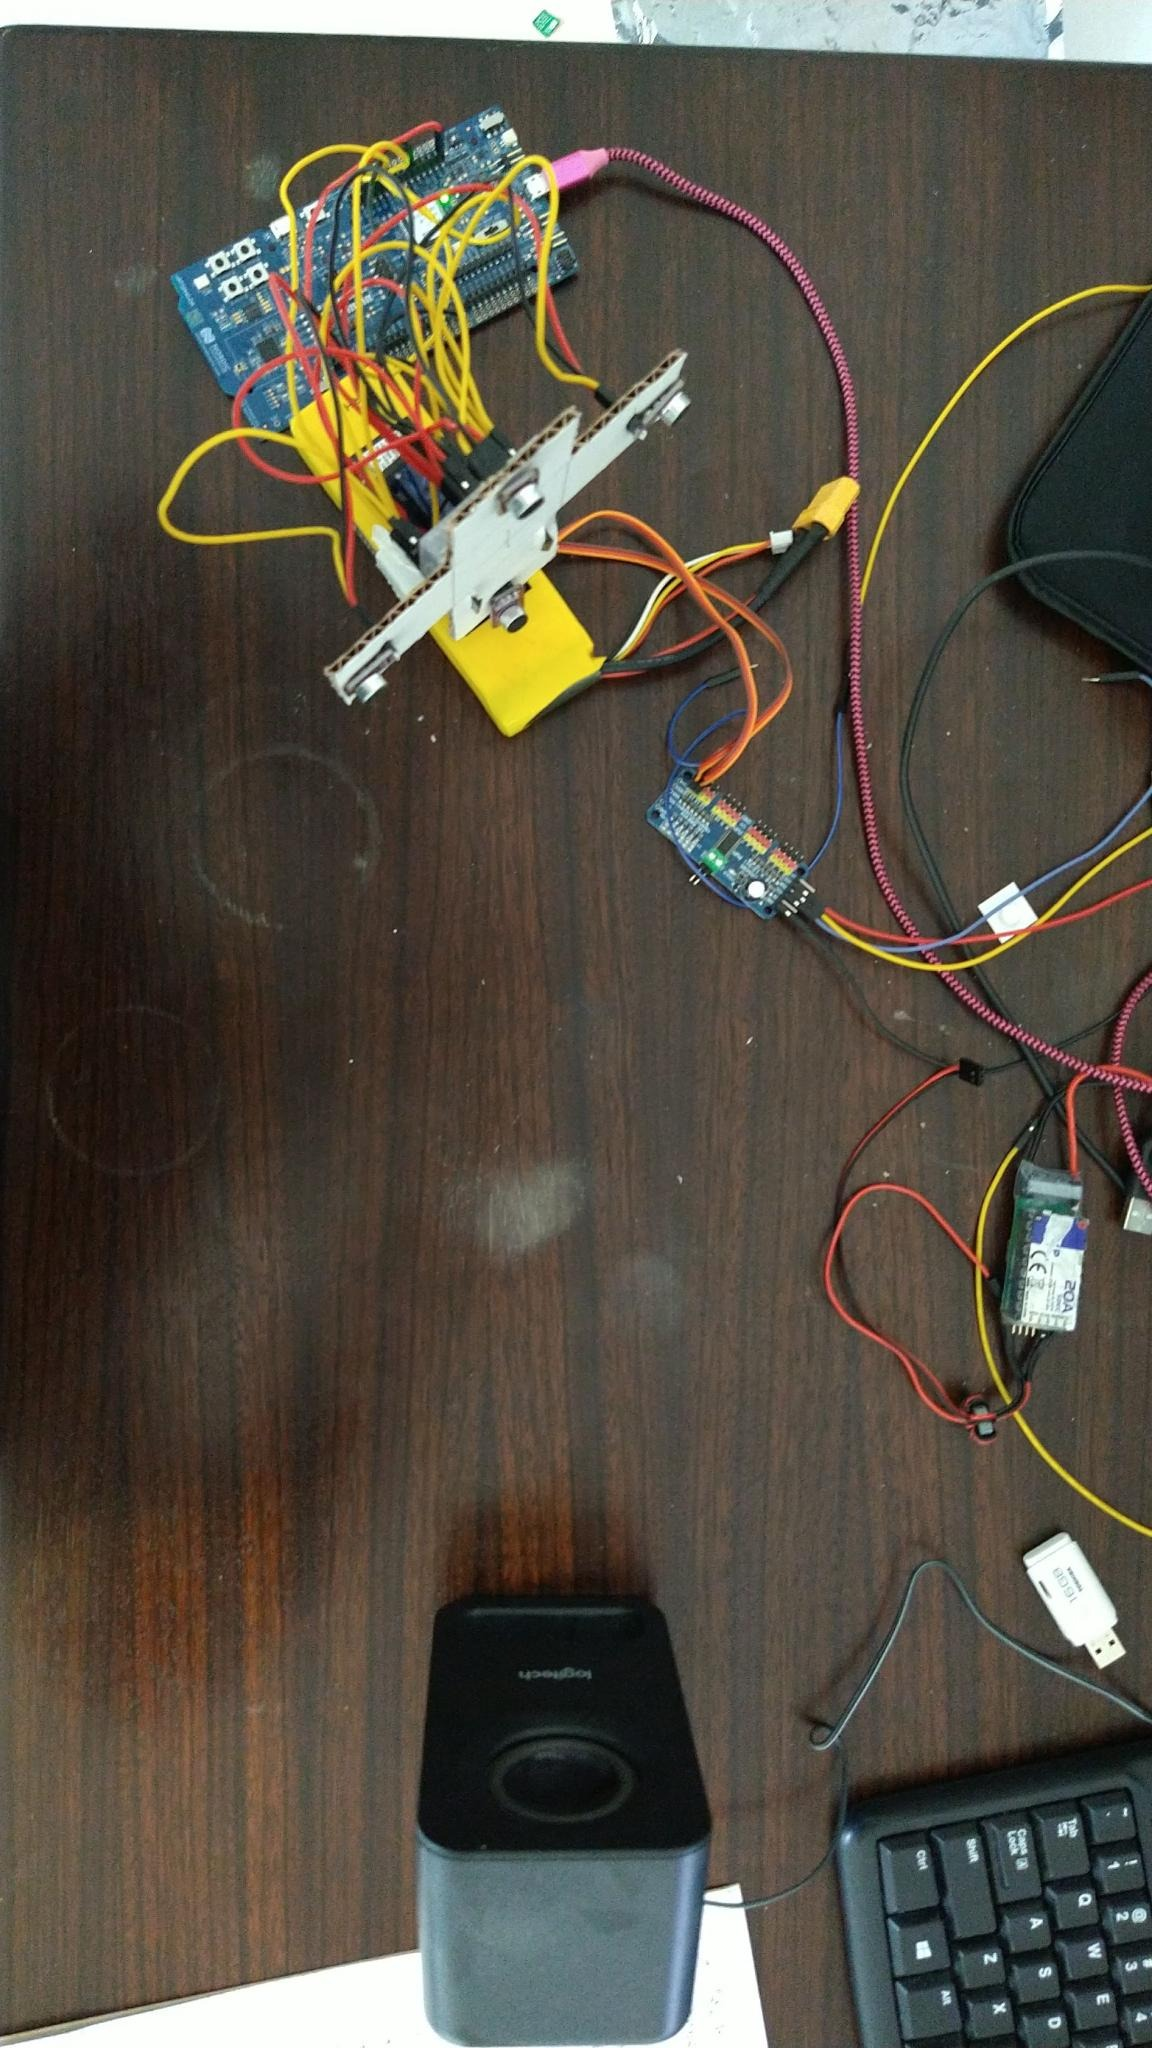
\includegraphics[angle=90,width=\linewidth]{assets/test_setup.jpeg}
        \caption{Setup for taking measurements}
        \label{fig:test_setup}
    \end{center}
\end{figure}

\begin{listing}[H]
    \begin{minted}[autogobble]{matlab}
        function [ ...
        N, ...
        avg, ...
        passed_samples, ...
        pass_percentage, ...
        passed ...
    ] = analyze_measurements(file_path, expected_angle) 
            [~, name, ext] = fileparts(file_path);
            file_basename = sprintf("%s%s", name, ext);
            samples = readmatrix(file_path);
            N = length(samples);
            avg = mean(samples);
            std_dev = std(samples);

            passed_samples = 0;
            for x = samples'
                if abs(x - expected_angle) < 10
                    passed_samples = passed_samples + 1;
                end 
            end

            pass_percentage = (passed_samples/N) * 100;
            passed = mat2str(pass_percentage > 80);

            fprintf("Number of samples:\t%d\n", N);
            fprintf("Average value:\t\t%g°\n", round(avg, 2))
            fprintf("Standard deviation:\t%g\n", round(std_dev, 2))
            fprintf("Percent within range:\t%g%%\n", round(pass_percentage, 2));
            fprintf("Pass:\t\t\t%s\n", passed);
            
            % snip
        end
    \end{minted}
        \caption{\texttt{analyze\textunderscore measurements.m} Matlab script}
        \label{list:analyze_measurements}
    \end{listing}
    
\section{Results and Analysis}
% Evaluation of the results using the defined criteria and a reflection on the outcomes, explanations for shortcomings, ideas for improvements.

The results of the evaluation are shown in the tables below. In table \ref{tab:results_baseline}, the results for the baseline measurement without any sound are shown. In the table, the value of N is the amount of calculation outputs that were analyzed. In other words, the device took N times 1024 samples from the horizontal microphones, cross correlated the signals, and calculated the corrresponding angle from it. Without any sound playing, the device detects an angle of $90^{\circ}$ with a standard deviation of $0$. As there was no expected angle, data on passing the test was recorded.

% baseline
\begin{table}[H]
    \begin{center}
        \begin{tabular}{ | m{5em} | m{2em} | m{3.5em} | m{3.5em} | }
            \hline
            File name    & N   & Average ($^{\circ}$) & Standard deviation \\
            \hline
            \hline
            baseline.txt & 101 & 90                   & 0                  \\
            \hline
        \end{tabular}
        \caption{Results from testing with 1100Hz sine wave signal.}
        \label{tab:results_baseline}
    \end{center}
\end{table}

In table \ref{tab:results_sine1100hz}, the results of analyzing the $1100\ Hz$ sine wave are shown. Only at angles $\theta = 45^{\circ}$ and $\theta = 90^{\circ}$, the test passes. For the other angles, the pass percentage is $0 \%$, meaning none of the outputs were within $10^{\circ}$ of the expected angle. The standard deviation is $0$ or almost $0$ for all angles, meaning that the calculations done by the device are consistent when presented a sine wave of $1100\ Hz$. Overall, however, the device does not meet the evaluation criteria.

% sine_1100hz
\begin{table}[H]
    \begin{center}
        \begin{tabular}{ | m{5em} | m{4em}| m{2em} | m{3.5em} | m{3.5em} | m{3.5em} | m{3.5em} | m{2.5em} | }
            \hline
            File name                  & Expected angle ($^{\circ}$) & N   & Average ($^{\circ}$) & Standard deviation & Passed samples & Pass percentage & Test passed \\
            \hline
            \hline
            0\textunderscore deg.txt   & 0                           & 101 & 24                   & 0                  & 0              & 0 \%            & false       \\
            \hline
            45\textunderscore deg.txt  & 45                          & 101 & 53                   & 0                  & 101            & 100 \%          & true        \\
            \hline
            90\textunderscore deg.txt  & 90                          & 101 & 90                   & 0                  & 101            & 100 \%          & true        \\
            \hline
            135\textunderscore deg.txt & 135                         & 101 & 114.42               & 1.66               & 0              & 0 \%            & false       \\
            \hline
            180\textunderscore deg.txt & 180                         & 101 & 156                  & 0                  & 0              & 0 \%            & false       \\
            \hline
        \end{tabular}
        \caption{Results from testing with 1100Hz sine wave signal.}
        \label{tab:results_sine1100hz}
    \end{center}
\end{table}

Table \ref{tab:results_mosquito} lists the results of analyzing the mosquito sound. Again, only two angles are estimated sufficiently, and the evaluation criteria are not met. We can see that the sandard deviation for the mosquito sounds are high at the extreme values for $\theta$, but goes to zero as $\theta$ comes closer to $90^{\circ}$.

% mosquito
\begin{table}[H]
    \begin{center}
        \begin{tabular}{ | m{5em} | m{4em}| m{2em} | m{3.5em} | m{3.5em} | m{3.5em} | m{3.5em} | m{2.5em} | }
            \hline
            File name                  & Expected angle ($^{\circ}$) & N   & Average ($^{\circ}$) & Standard deviation & Passed samples & Pass percentage & Test passed \\
            \hline
            \hline
            0\textunderscore deg.txt   & 0                           & 101 & 32.07                & 20.21              & 0              & 0 \%            & false       \\
            \hline
            45\textunderscore deg.txt  & 45                          & 101 & 56.29                & 8.24               & 75             & 74 \%           & false       \\
            \hline
            90\textunderscore deg.txt  & 90                          & 101 & 90                   & 0                  & 101            & 100 \%          & true        \\
            \hline
            135\textunderscore deg.txt & 135                         & 101 & 128.72               & 11.03              & 91             & 90 \%           & true        \\
            \hline
            180\textunderscore deg.txt & 180                         & 101 & 146                  & 22.81              & 0              & 0 \%            & false       \\
            \hline
        \end{tabular}
        \caption{\label{tab:results_mosquito}Results from testing with mosquito sound.}
    \end{center}
\end{table}


\section{Conclusions}
% (Short) What did you learn from doing the project? What solutions did you provide?


\bibliographystyle{plain}
\bibliography{references}
\end{document}
